
\documentclass[conference]{IEEEtran}

\usepackage{hyperref}
\usepackage{amsmath}
\usepackage{amssymb}
\usepackage{hhline} % easy to manage table borders
\usepackage{colortbl} % colored cells in tables
\usepackage{multirow}
\usepackage{enumerate}
\usepackage{slashbox} % cell with slash inside
\usepackage{makeidx}  % allows index generation
\usepackage[utf8]{inputenc}
\usepackage{graphicx}
\usepackage{setspace}

\newtheorem{definition}{Definition}
\newtheorem{example}{Example}

\def\sectionautorefname{Section}
\def\subsectionautorefname{Section}

\begin{document}
%
% paper title
% can use linebreaks \\ within to get better formatting as desired
\title{Semantic Medical Prescriptions -- Towards Intelligent and Interoperable Medical Prescriptions}


% author names and affiliations
% use a multiple column layout for up to three different
% affiliations
%PO 100920, D-04009 Leipzig\\
\author{\IEEEauthorblockN{Ali Khalili}
\IEEEauthorblockA{Institute of Informatics\\
University of Leipzig, Germany\\
khalili@informatik.uni-leipzig.de}
\and
\IEEEauthorblockN{Bita Sedaghati}
\IEEEauthorblockA{Institute of Pharmacy\\
University of Leipzig, Germany\\
bita.sedaghati@uni-leipzig.de}
}

% make the title area
\maketitle


\begin{abstract}
Medication errors are the most common type of medical errors in health-care domain.
The use of electronic prescribing systems (e-prescribing) have resulted in significant reductions in medication errors.
However, one of the main challenges in e-prescription systems is handling heterogeneity of available information sources.
There exist already different sources of information addressing different aspects of pharmaceutical research (e.g. chemical, pharmacological and pharmaceutical drug data, clinical trials, approved prescription drugs, drugs activity against drug targets. etc.).
Handling these dynamic information within current e-prescription systems without blurring the border of the existing pharmaceutical information islands is a cumbersome task.
The recent proliferation of Linked Open Data that enables the integration of multiple disparate data sources proposes a solution to this problem.
In the domain of pharmaceutical research, many efforts have been done to create a linked open drug data.
In this paper we present the Pharmer as an approach to employ Linked Open Data to facilitate the creation of semantic medical prescriptions.
Semantic prescriptions are intelligent e-prescription documents enriched by drug-related meta-data thereby know about their content and the possible interactions.
Semantic prescriptions provide an interoperable interface which helps patients, physicians, pharmacists, researchers and companies to collaboratively improve the quality of pharmaceutical services by facilitating the process of shared decision making.
%Pharmer provides different views for the different personas involved in the process of e-prescribing.
Pharmer employs datasets such as DBpedia, DrugBank, DailyMed and RxNorm to automatically detect the drugs in the prescriptions and to collect multidimensional data on them.
It also warns of the possible drug interactions in the prescription.
We evaluate the feasibility of the Pharmer by conducting a usability evaluation and report on the quantitative and qualitative results of our survey.
\end{abstract}

\begin{IEEEkeywords}
 Semantic prescription; e-prescription; semantic annotation; e-health;

\end{IEEEkeywords}

\IEEEpeerreviewmaketitle


\section{Introduction}
\label{intro}

As reported in MedicineNet~\cite{medicationErrors}, \emph{medication errors} are the most common type of medical errors in health care.
Errors such as improper dose of medicine, adverse drug interactions, food interactions, etc. often stem from invalid prescriptions and unawareness of the patients.
Electronic prescriptions which are recently gaining attention in the e-health domain, are one of the solutions proposed to solve these type of errors.
While even nowadays traditional paper prescriptions are commonly used, e-prescriptions offer several advantages.
In an e-prescription system, prescriber electronically sends an accurate, error-free and understandable prescription directly to a pharmacy from the point-of-care.
Reduction in medication error and decline in adverse drug events are more highlighted consequences of e-prescribing.

During the recent years, the adoption of e-prescriptions has been spreading rapidly.
To illustrate, the Australian government started launching of e-prescription from March 2007~\cite{medicare}.
Using this system, the e-providers who effectively market themselves on the web will have a distinct advantage.
A system called epSOS~\cite{epsos} which performs the use of e-prescriptions all around Europe, is currently passing the extensive practical testing phase.
epSOS contains patient summary and an e-prescription service which allows access to the cross-border e-health services.
This service allows people in participating epSOS pilot countries, as tourists, business travellers, commuters or exchange students to take advantage of e-health services.
The e-prescribing incentive program performed in US~\cite{epincentive} is another example in this area.
As a reporting program it uses a combination of incentive payments and payment adjustments to encourage electronic prescribing by eligible professionals.

One of the main challenges of e-prescription systems is the heterogeneity of available information sources.
There exist already different sources of information addressing different aspects of pharmaceutical research.
Information about chemical, pharmacological and pharmaceutical drug data, clinical trials, approved prescription drugs, drugs activity against drug targets such as proteins, gene-disease-drug associations, adverse effects of marketed drugs, etc. are some examples of these diverse information.
Handling these dynamic information within current e-prescription systems without blurring the border of the existing pharmaceutical information islands is a cumbersome task.
On the other hand, \emph{Linked Open Data} as an effort to interlink and integrate these isolated sources of information is obtaining more attention in the domain of pharmaceutical, medical and life sciences.

Combining the best practices from Linked Open Data together with e-prescription systems can provide an opportunity for patients, researchers as well as practitioners to collaborate together in a synergic way.
A consequence of introducing linked data in health care sector is that it significantly changes the daily duties of the employees of the health care sector.
Therefore the most challenging aspect will not be the technology but rather changing the mind-set of the employees and the training of the new technology\cite{challengesEP}.
Furthermore, the information generated via that approach can be employed as a data source for researchers.
Drug companies are also able then to take the advantage of considering these informative statistical data.

Semantic prescriptions as introduced in this paper are a proposed approach to utilize semantic web technologies in e-prescription systems.
As intelligent prescriptions, they can automatically handle the medical errors occurring in prescriptions and increase the awareness of the patients about the prescribed drugs and drug consumption in general.
Semantic prescriptions also enable the creation of more efficient and effective search approaches for drug discovery and consumption.
We created a tool called \emph{Pharmer} as a showcase application to facilitate the process of semantic prescription generation.
Pharmer adopts a bottom-up approach for enriching the normal e-prescriptions with semantic annotations using a set of predefined datasets from linked open data.

The remainder of this article is structured as follows:
\autoref{sec:lod}, \autoref{sec:sca} and \autoref{sec:epresc} provide a background on the basic concepts such as Linked Open Data, Semantic Content Authoring and E-prescriptions employed in this paper.
In \autoref{sec:pharmer}, we describe the Pharmer as a solution to effectively create semantic prescription.
Then we discuss the possible benefits of Pharmer in \autoref{sec:stake}.
To better clarify the use cases of the Pharmer system, an example scenario is drawn in \autoref{sec:example}.
In \autoref{sec:evaluation}, Pharmer usability evaluation results are reported and finally \autoref{sec:conclusion} concludes with an outlook on future work.

\section{Linked Open Data}
\label{sec:lod}
In computing, \emph{Linked Data} describes a method of publishing structured data so that it can be interlinked and become more useful.
It builds upon standard Web technologies such as HTTP and URIs, but rather than using them to serve web pages for human readers, it extends them to share information in a way that can be read automatically by computers.
This enables data from different sources to be connected and queried \cite{linkeddata}.
Tim Berners-Lee, the inventor of the Web and Linked Data initiator, suggested a 5 star deployment scheme for \emph{Linked Open Data}:
1) make your stuff available on the Web (whatever format) under an open license,
2) make it available as structured data (e.g., Excel instead of image scan of a table),
3) use non-proprietary formats (e.g., CSV instead of Excel),
4) use URIs to identify things, so that people can point at your stuff,
5) link your data to other data to provide context.

\begin{figure}[tb]
	\centering
		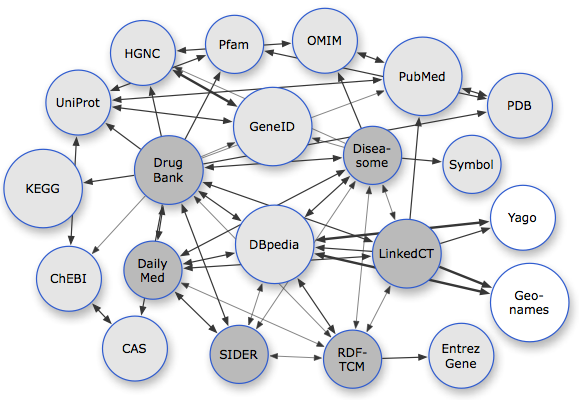
\includegraphics[width=1.0\columnwidth]{../images/lod_cloud.png}
	\caption{Available datasets related to pharmaceutical research.}
	\label{fig:lod}
\end{figure}

Particularly in the areas of health care and life sciences with the wealth of available data, large scale integration projects like Bio2RDF~\cite{bio2rdf}, Chem2Bio2RDF~\cite{chembio}, and the W3C HCLS’s (Health Care and Life Sciences) Linked Open Drug Data (LODD)\cite{lodd} have not only significantly contributed to the development of the Linked Open Data effort, but have also made social and technical contributions towards data integration, knowledge management, and knowledge discovery.

There are already many interesting information on pharmaceutical research available on the Web.
The sources of data range from drugs general information, interactions and impacts of the drugs on gene expression, through to the results of clinical trials.
LODD\cite{lodrug} has surveyed publicly available data about drugs, created Linked Data representations of the data sets, and identified interesting scientific and business questions that can be answered once the data sets are connected.

One of the use cases of LODD datasets is authoring of \emph{Semantic Prescriptions} which are prescriptions enriched by linked open data.

\section{Semantic Content Authoring}
\label{sec:sca}
 A \emph{Semantic Document} is an intelligent document (with explicit semantic structure) which ``knows about" its own content so that it can be automatically processed in unforeseen ways.
Semantic documents facilitate a number of important aspects of information management~\cite{rdface}.
For \emph{search and retrieval}, they provide more efficient and effective search interfaces, such as faceted search~\cite{tunkenlang2009faceted} or question answering~\cite{Lopez2011}.
In \emph{information presentation}, they support more sophisticated ways of flexibly visualizing information, such as by means of semantic overlays as described in~\cite{Burel2009}.
In \emph{information integration}, they provide unified views on heterogeneous data stored in different applications by creating composite applications such as semantic mashups~\cite{Ankolekar2007}.
For \emph{personalization}, they provide customized and context-specific information which better fits user needs and will
result in delivering customized applications such as personalized semantic portals~\cite{ecs2007}.
For \emph{reusability} and \emph{interoperability}, they facilitate exchanging content between disparate systems and enabling applications such as executable papers~\cite{Muller2011}.


The above benefits, however, come at the cost of increased authoring effort. %~\cite{hasida2007,uren2006}
A \emph{Semantic Authoring User Interface} is a human accessible interface with capabilities for writing and modifying semantic documents which are either.
\emph{Semantic Content Authoring} (SCA) is a tool-supported manual composition process aiming at the creation of semantic documents which are either:
\begin{itemize}
	\item fully semantic in the sense that their original data model uses a semantic knowledge representation formalism (such as RDF, RDF-Schema or OWL) or
	\item based on a non-semantic representation form (e.g. text or hypertext), which is enriched with semantic representations during the authoring process.\\
\end{itemize}

With an ontology and a user interface appropriate for the type of content, semantic authoring can be easier than traditional composition of content and the resulting content can be of higher quality~\cite{hasida2007}.

Medical prescriptions are a good candidate to be enriched by semantic annotations.
Semantic prescriptions enable the traditionally written prescriptions to be utilized in novel ways as discussed above.
In the following sections, we first describe the e-prescriptions and then discuss how they can be enriched as semantic documents.

\section{e-prescriptions}
\label{sec:epresc}
E-health has evolved and emerged recently in many forms.
E-prescription is one of those forms and defined as a computer-generated prescription utilized by health-care providers.
E-prescribing as it is commonly called, is the use of an automated data entry system to generate a prescription that is then transmitted through a special network to a pharmacy in such a way that the data goes directly into the pharmacy’s computer system.
It plays an important role in improving the quality of patient care.
For the prescriber, e-prescribing happens when a physician uses a computer or handheld device with a software that allows him or her to (with the patient’s consent) electronically access information regarding a patient’s drug benefit coverage and medication history; electronically transmit the prescription to the patient’s pharmacy of choice; and, when the patient runs out of refills, his or her pharmacist can also electronically send a renewal request to the physician’s office for approval.

In order to see an increase in both quality and efficiency that can be attributed to e-prescribing, the system must be capable of performing key functions related to:
\begin{itemize}
  \item Medication selection/decision support capabilities (e.g., diagnosis-based medication menus, evidence based information, drug interaction checking, safety-alerts, formulary checking, prescription renewal, and dosage calculation).
  \item Patient-specific information capabilities (e.g., current patient medication list, access to patient historical data, patient identification).
  \item System integration capabilities (e.g., connection with various databases, connection with pharmacy and pharmacy benefit manager systems).
  \item Educational capabilities (e.g., patient education, provider feedback).
\end{itemize}


One of the main challenges of the current e-prescription systems is the heterogeneity and evolving nature of available information sources.
There exist already different sources of information addressing different aspects of pharmaceutical research.
Handling these dynamic information within current e-prescription systems without blurring the border of the existing pharmaceutical information islands is a cumbersome task.

\section{Pharmer: Semantic Authoring of Medical Prescriptions}
\label{sec:pharmer}
Pharmer is an application created as a proof of concept for the authoring of semantic prescriptions.
The Pharmer implementation is open-source and available for download together with an explanatory video and online demo at \cite{pharmerproject}.
Pharmer adopts a bottom-up approach~\cite{khalili2012} for enriching the normal e-prescriptions with semantic annotations using a set of predefined ontologies.

\begin{figure}[tb]
	\centering
		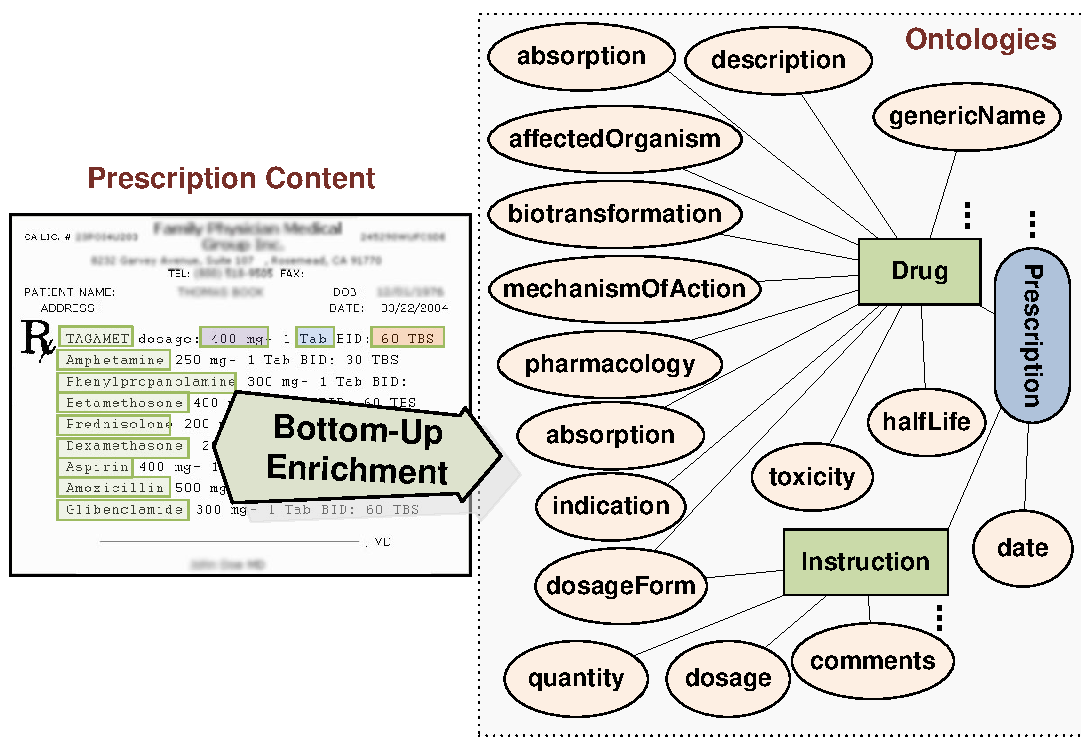
\includegraphics[width=1.0\columnwidth]{../images/approaches.pdf}
	\caption{Bottom-up semantic enrichment of prescriptions.}
	\label{fig:botup}
\end{figure}

The basic ingredients of a semantic annotation system are ontologies, the documents and the annotations that link ontologies to documents~\cite{khalili2012}.
Here, we need two kinds of ontologies:
\emph{Annotation ontologies} (i.e. metadata schemata) which define what kind of properties and value types should be used for describing a resource.
\emph{Domain ontologies} which are used to define vocabularies providing possible values for metadata properties.
We use \url{Schema.org} MedicalTherapy vocabulary as our annotation ontology and utilize the existing pharmaceutical linked datasets such as DBpedia, DrugBank, DailyMed and RxNorm as our domain ontology.


\subsection{Architecture}

The Pharmer system architecture is depicted in \autoref{fig:arch} and consists of three layers:

\begin{figure}[tb]
	\centering
		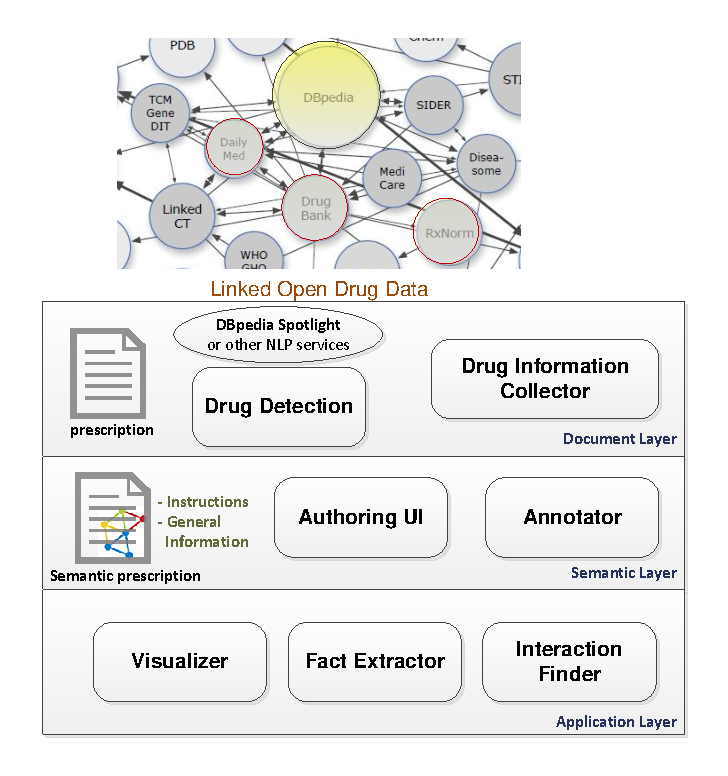
\includegraphics[width=1\columnwidth]{../images/architecture.pdf}
	\caption{Architecture of the Pharmer system.}
	\label{fig:arch}
\end{figure}

\paragraph{Document Layer} This layer includes the traditional e-prescription document plus two components as \emph{Drug Detection} and \emph{Drug Information Collector}.
Drug detection component performs the natural language processing (NLP) of the e-prescription document to detect the terms referring to a drug in the prescription.
The component uses DBpedia spotlight~\cite{dbspotlight} and BioPortal annotator~\cite{bioportal} NLP services to parse and analyze the text looking for known drugs.
It is configurable so that users can easily add other existing NLP services for drug detection.
When user is writing the prescription, this component asynchronously performs the drug recognition and adds the related annotations as real-time semantic tagging.

Another component in this layer is drug information collector which grabs all the information regarding a specific drug from Linked Open Data.
To pursue this, it utilizes datasets such as DrugBank, DailyMed and RxNorm (available at \cite{lodd}) by sending federated SPARQL queries.

\paragraph{Semantic Layer}
There are two main components in this layer namely \emph{Annotator} and \emph{Authoring UI}.
The \emph{annotator} component handles the automatic annotation and embeds the general information of the drugs as meta-data into the e-prescription.
Annotator adopts the RDFa format. \emph{RDFa} (Resource Description Framework in attributes) is a W3C Recommendation that adds a set of attribute level extensions to XHTML for embedding RDF metadata within web documents.
RDFa fulfills the principles of interoperable metadata such as publisher independence, data reuse, self containment, schema modularity and evolvability.

The \emph{authoring UI} component provides users with a set of input forms to manually embed the meta-data related to prescription instructions into the prescription document.

\paragraph{Application Layer}
This layer provides a set of applications on top of the generated semantic prescriptions.
\emph{Interaction Finder} checks the possible interactions between the prescribed drugs and warn the prescriber about them.
\emph{Visualizer} is responsible for graphically representing the embedded semantics of a prescription (e.g. as depicted in \autoref{fig:graphview}).
The \emph{Fact Extractor} generates the RDF/Turtle representation of the semantic prescriptions (e.g. as depicted in \autoref{fig:factview}).

\subsection{Features}
The main features of Pharmer can be summarized as:
\begin{itemize}
	\item \emph{Providing Different Semantic Views}.
	Semantic views allow the generation of different views on the same metadata schema and aggregations of the knowledge base based on the roles, personal preferences, and local policies of the intended users.
	Pharmer suggests two types of views: generic and domain specific views.
	Generic views provide visual representations of drug information (e.g. as information view depicted in \autoref{fig:screenshot} or graph view\autoref{fig:graphview}.
	Domain specific views address the requirements of a particular domain user (e.g. a researcher need specific views for visualizing the atomic structure of chemical compounds).
	\item \emph{Real-time Drug Tagging.}
	Real-time tagging means creating drug annotations while the user is typing.
	This will significantly increase the annotation speed~\cite{OCA}.
	Users are not distracted since they do not have to interrupt their current authoring task.
	Pharmer has a client-side component which interacts with the server asynchronously to make real-time tagging possible.
	\item \emph{Drug Suggestion.}
		When searching for a drug, Pharmer suggests the similar drugs by taking into account the history of search terms.
    \item \emph{Automatic Drug Annotation.}
    Automatic annotation means the provision of facilities for automatic mark-up of prescriptions.
    The automatic process of annotating in Pharmer is composed basically of finding drug terms in prescription using an NLP service, mapping them against an ontology, and disambiguating common terms.
\end{itemize}



\begin{figure*}[tb]
	\centering
		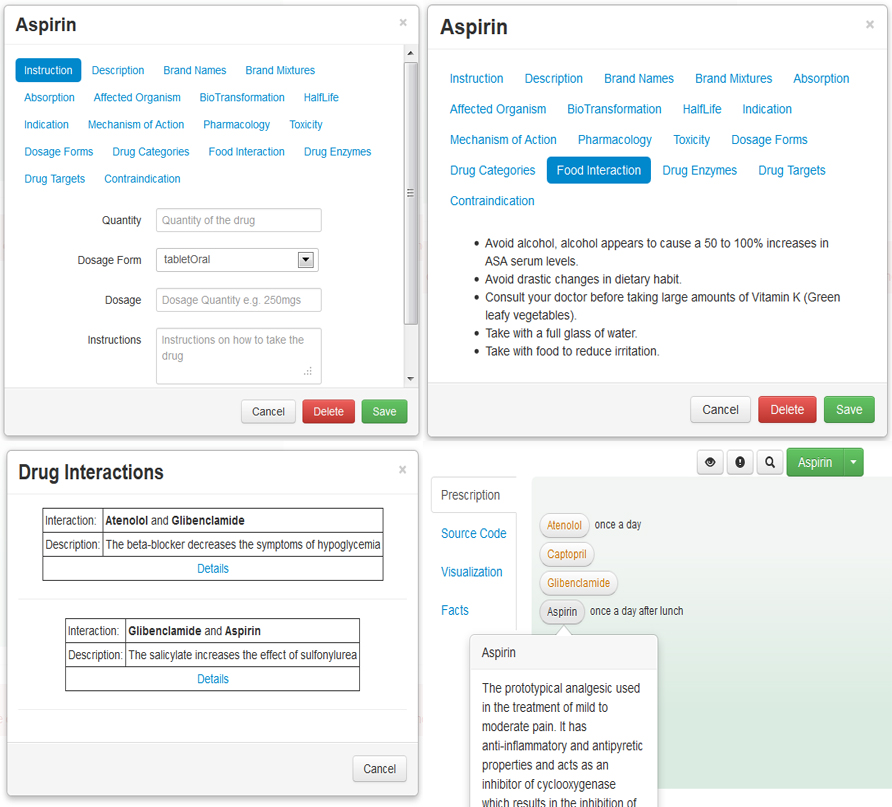
\includegraphics[width=1\textwidth]{../images/screenshot1.jpg}
	\caption{Screenshot of the Pharmer applicatpion.}
	\label{fig:screenshot}
\end{figure*}

\begin{figure}[tb]
	\centering
		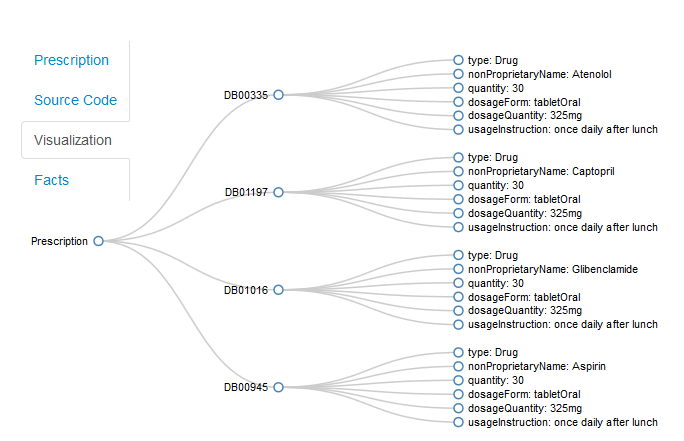
\includegraphics[width=1\columnwidth]{../images/sc2.png}
	\caption{Graph view.}
	\label{fig:graphview}
\end{figure}

\begin{figure}[tb]
	\centering
		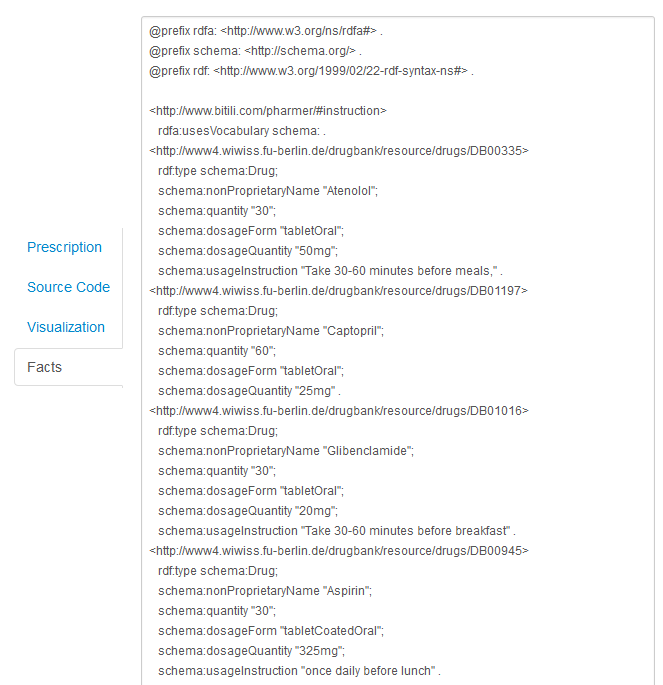
\includegraphics[width=1\columnwidth]{../images/sc4.png}
	\caption{Fact view.}
	\label{fig:factview}
\end{figure}

\subsection{Pharmer Stakeholders}
\label{sec:stake}

As depicted in \autoref{fig:system}, Pharmer approach is very versatile and can be applied in a vast number of use cases by different stakeholders. The arrows in the figure can be summarized as the following:

\begin{enumerate}
\item The physician diagnoses the disease and writes the corresponding semantic prescription using the Pharmer. The patient's medication history is available to the physician as well.
\item Pharmer utilizes the Linked Open Data as its integrated information source.
\item The researcher can analyze the stored semantic prescriptions data.
\item Drug companies utilize the Pharmer data store in order to balance their production and distribution according to the market taste and demand.
\item The pharmacist verifies the prescription and hands in the medication to the patient.
\item The patient inquires drug information and can contact the related physician and pharmacist.
\end{enumerate}

The main benefit of using semantic prescriptions is the persistent connection to up-to-date drug information coming from multiple dynamic data sources.
So, when a change occurs to a drug (e.g. change in its effects or interactions) the semantic prescription automatically adopts to this new change.
Once writing a prescription it is very critical to consider drug interactions.
Drug interactions are divided to three categories namely \emph{food-drug}, \emph{drug-drug} and \emph{drug-plant} interactions.
Coadministration can either be synergistic or antagonistic which respectively increase or decrease the drugs effect.
The interactions may sometimes lead to change in the drug effect.
By applying semantic prescriptions, all types of drug interactions are prevented and the probability of errors in prescriptions are reduced to a great extend.

A semantic prescription is a self-contained document which is aware of its content and is connected to the linked open data.
In contrast to database-oriented e-prescriptions, semantic prescriptions can easily be exchanged among other e-health systems without need to changing their related infrastructure hence enabling a connection between physicians, pharmacists, patients, pharmaceutical researchers and drug companies.

Furthermore, semantic prescriptions increase the awareness of patients.
They provide patients with all the related information of the prescribed drugs thereby mitigating the possible misuse of drugs.
In addition, semantic prescriptions support shared decision making (SDM) by allowing patients and service providers to make health care decisions together.
They connect the best scientific evidence available with the patient’s values and preferences.

It brings the following benefits for its stakeholders:
\begin{itemize}
\item Physicians: increased efficiency, improved care, patient satisfaction and potential short and long-term incentives.
\item Patients: increased information, safety, efficiency and compliance.
\item Pharmacists: increased efficiency, improved service quality, improved patient satisfaction,  prevention of adverse drug reactions and speeding up the whole process.
\item Researchers: easy accessed abundant information source and statistical data availability.
\item Drug companies: production efficacy, patient compliance and rate of the consumption of each medicine.
\end{itemize}

\begin{figure}[tb]
	\centering
		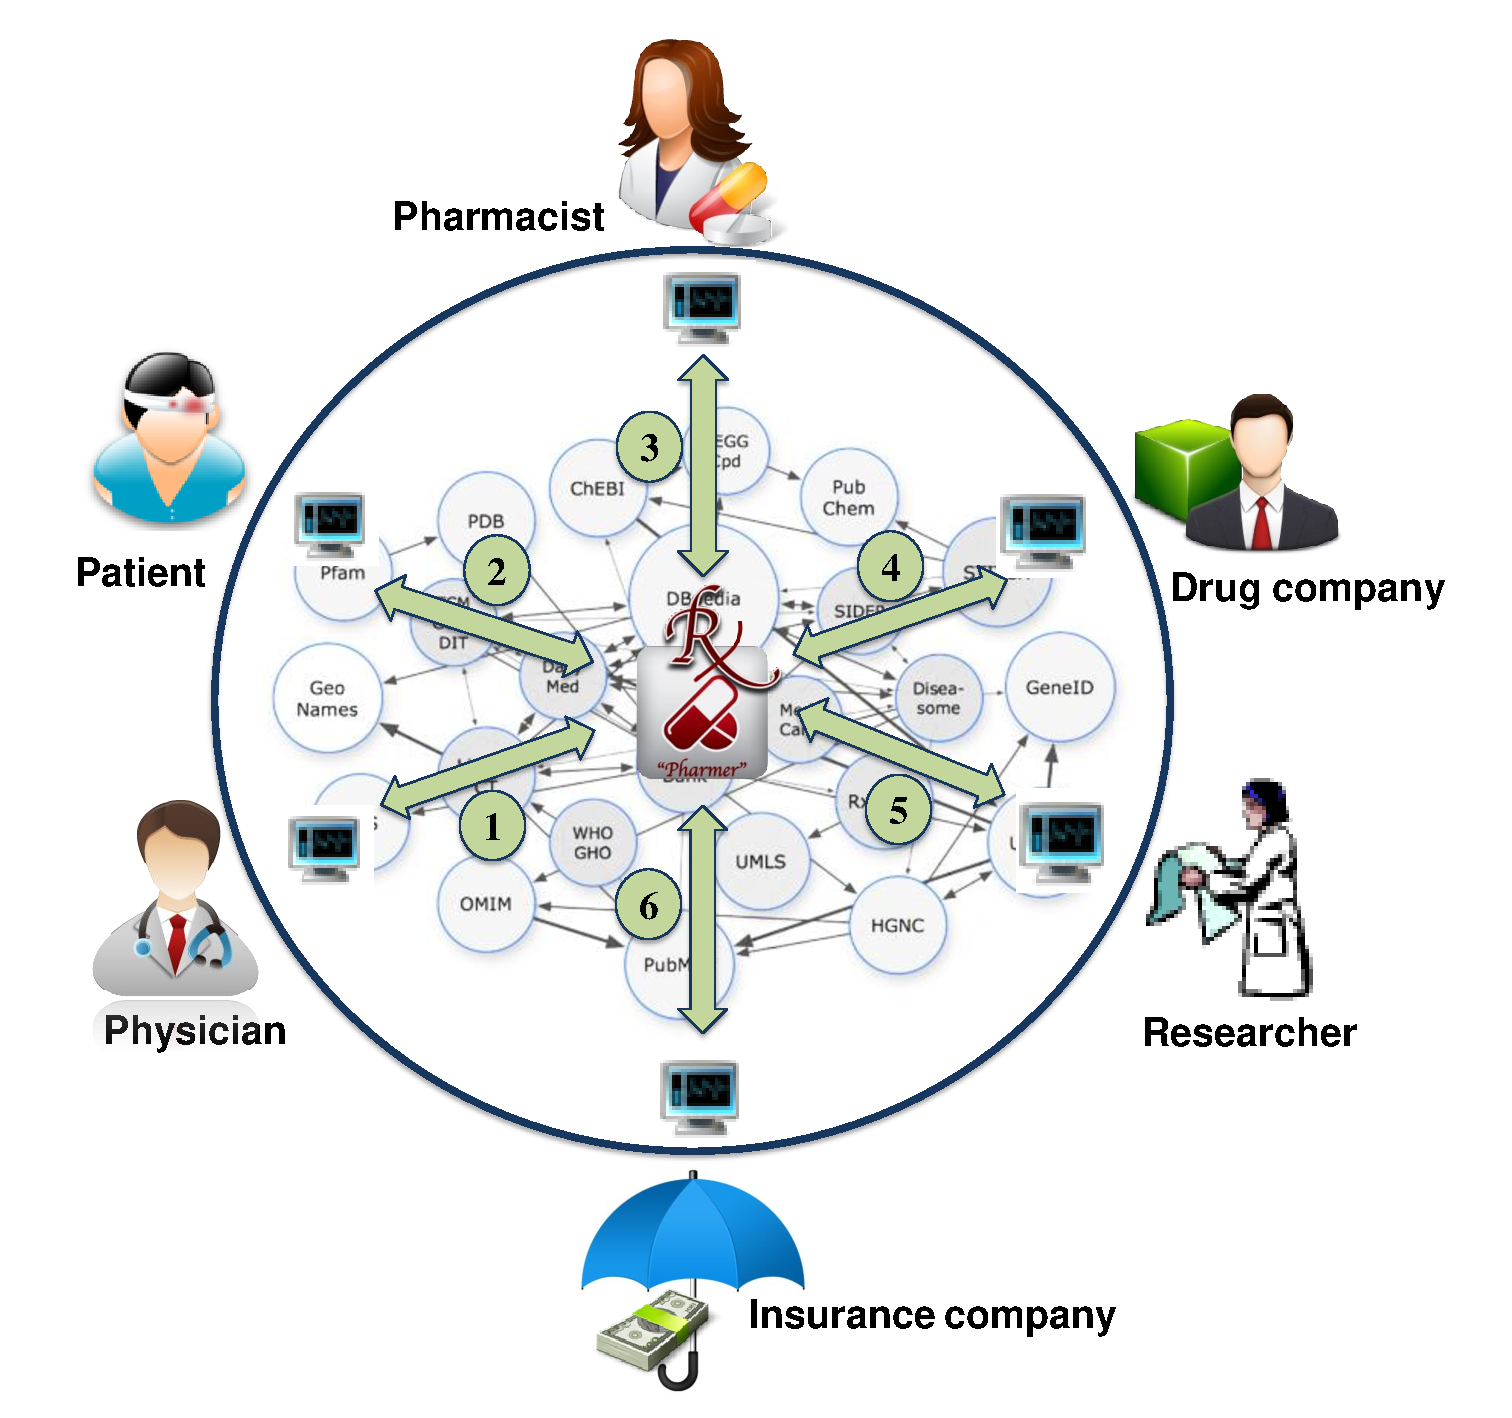
\includegraphics[width=1.0\columnwidth]{../images/system.pdf}
	\caption{Pharmer ecosystem.}
	\label{fig:system}
\end{figure}

\section{Example scenario}
\label{sec:example}
As a scenario; a 63 year old man with the history of MI (Myocardial Infarction) and type 2 diabetes visits a heart and coronary specialist complaining about frequent headaches and heavy head feeling. The specialist, after general inspection and monitoring vital signs, asks for a blood test.
He then considers symptoms including high blood pressure (sys/dias:158/95 mmHg) and high Fasting Blood Sugar (150 mg/dl).
He diagnoses high blood pressure plus severe type 2 diabetes.
Thereby, The patient profile is defined in Pharmer by patient's information besides diagnosis.
``no weight loss" is mentioned as a preference in the patient's profile.
Regardless of the patient's preferences, the physician would prescribe \texttt{Metformin} as a drug of choice.
However, since the major side effect of \texttt{Metformin} is weight loss, the physician replaces \texttt{Metformin} with \texttt{Rosiglitazone}.
Considering the medication that the patient took before (\texttt{Glibenclamide} only), The specialist dispenses a new semantic prescription by entering the following drugs:

\begin{itemize}
\item \textbf{Rosiglitazone} 4 mg Oral Tablet once daily
\item \textbf{Glibenclamide} 5 mg Oral Tablet bid
\item \textbf{Atenolol} 50 mg Oral Tablet once daily
\end{itemize}

He then checks for the possible drug interactions by clicking the attributed button in the Pharmer software.
As the Pharmer is connected to linked open data it is capable of recognizing the most recent updated drug interactions.
He finds out that Sulfunyl Urea class drugs (here \texttt{Glibenclamide}) are not compatible to be coadministrated with beta-blockers (here \texttt{Atenolol}).
So, he needs to replace it with another drug.
Using the Pharmer and its connection to linked open data, the physician can find the possible alternatives.
Then he decides to choose \texttt{Captopril} as replacement.
The semantic prescription is then sent to the patient's pharmacy of choice.
There, pharmacist is able to review the semantic prescription and comments on that directly in the system so that the physician is also aware of the corresponding changes.
Pharmacist comments may cause minor or major modifications in the semantic prescription.
For instance, using the Pharmer she is able to check the appropriate dose of each medicine or suggest cheaper alternatives (if possible).
In this case, as the \texttt{Rosiglitazone} elevates cardiovascular risks, the pharmacist suggests \texttt{Rosiglitazone} to be replaced by \texttt{Pioglitazone}.
This change happens as a realization of the shared decision making between physision, pharmacist and patient.
Thereafter, patient who was referred to the pharmacy takes the prescribed drugs.
Before he starts taking the tablets, he enters in Pharmer system with his ID as patient.
There, he is able to observe drug information embedded in the error free semantic prescription besides the preferred time and drug intake instructions.
He is also informed about the possible food interactions.
The patient's profile completes as he visits physicians or ask for refills.
Furthermore he is followed up by the physician and the pharmacist via the Pharmer.
After 2 months the patient visits another specialist for his recurrent symptoms of diabetes.
The specialist via the Pharmer accesses to the patient's medical profile and increases the anti-diabetic drug dose.

A researcher in an academy research institution investigates \texttt{Captopril} (as an Angiotansion II antagonist) effect on preventing diabetes recurrence.
Having the data from the aforementioned patient follow up along with other similar patients allows investigator to lead her goal.
In this case, for example, the \texttt{Captopril} along with anti-diabetic drugs led to diabetes recurrence.
Observing all the corresponding patient profiles will either confirm or reject the research assumption.

 A drug company manager requires to determine the compliance rate of \texttt{Captopril} in the market in order to balance the production based on market demand.
 Applying the Pharmer allows him to simply access to these data and decide how to go on with this product.
 He is also able to collect the evidence which may prevent further dispense of \texttt{Captopril} by physicians or consumption among patients.


\section{Evaluation}
\label{sec:evaluation}
In order to determine whether we succeeded to facilitate the creation of semantic prescriptions using Pharmer, we performed a usability user study with 13 subjects.
Subjects were drawn from 3 physicians, 4 pharmacist, 3 pharmaceutical researchers and 3 students.
We first showed them a tutorial video of using different features of Pharmer then asked each one to create a prescription with Pharmer.
After finishing the task, we asked the participants to fill out a questionnaire which consisted of two parts: feature usage questions and usability experience questions.

\begin{figure}[tb]
	\centering
		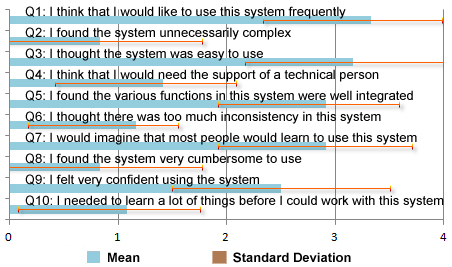
\includegraphics[width=1\columnwidth]{../images/pharmer_evaluation.jpg}
	\caption{Usability evaluation results for Pharmer (0: Strongly disagree, 1: Disagree, 2: Neutral, 3: Agree, 4: Strongly agree).}
	\label{fig:pharmerevaluation}
\end{figure}
We used the \emph{System Usability Scale} (SUS)~\cite{SUS2009} to grade the usability of Pharmer.
SUS is a standardized, simple, ten-item Likert scale-based questionnaire giving a global view of subjective assessments of usability.
It yields a single number in the range of 0 to 100 which represents a composite measure of the overall usability of the system.
The results of our survey (cf. \autoref{fig:pharmerevaluation}) showed a mean usability score of \textbf{75} for Pharmer which indicates a good level of usability.
Participants particularly liked the integration of functionality and the ease of learning and use.
The confidence in using the system was slightly lower, which we attribute to the short learning phase and diverse functionality.
Of course, this is a very simplified view on usability and we expect even better results could be achieved by putting more effort into the Pharmer development.
However, our goal was to demonstrate that Pharmer implementations with good usability characteristics can be created with relatively limited effort.
In addition to quantitative results, we also collected a number of user suggestions.
For instance some users suggested to provide a print-friendly document with all the patient's desired information.

\section{Conclusion}
\label{sec:conclusion}
Providing a consistent connection between patients, physicians, pharmacists, pharmaceutical researchers and drug companies is a crucial step towards enhancing the quality of knowledge management and thereby e-health services in the pharmaceutical domain.
With Pharmer, we presented in this article an approach for implementation of \emph{Semantic Prescriptions} as intelligent medical prescriptions to improve the integration and interoperability of e-prescribing systems with other e-health services.
Semantic prescriptions includes the important meta-data about the content of a prescription which will increase the awareness of their consumers.

We see the work presented in this article as an initial step in a larger research agenda aiming at promoting the authoring and annotation of semantically enriched medical documents.
Regarding future work, we envision to extend the Pharmer application towards different modalities, such that the annotation of images and other medical objects is supported.
Furthermore, we aim to integrate the other existing linked open datasets (e.g. related to publications, laboratories or insurance documents) into the Pharmer to extend its stakeholders.

%\clearpage

\bibliographystyle{IEEEtran}
\bibliography{../sca_refs,../refs}

% that's all folks
\end{document}


